\documentclass{standalone}
\usepackage{tikz}
\usetikzlibrary{patterns}
\usetikzlibrary{positioning}
\usetikzlibrary{patterns, positioning}
\usetikzlibrary{shapes.misc}
\usepackage[outline]{contour}
\contourlength{1.5pt} 
\usetikzlibrary{calc}
        \usepackage{relsize}
        \tikzset{fontscale/.style = {font=\relsize{#1}}}

\begin{document}
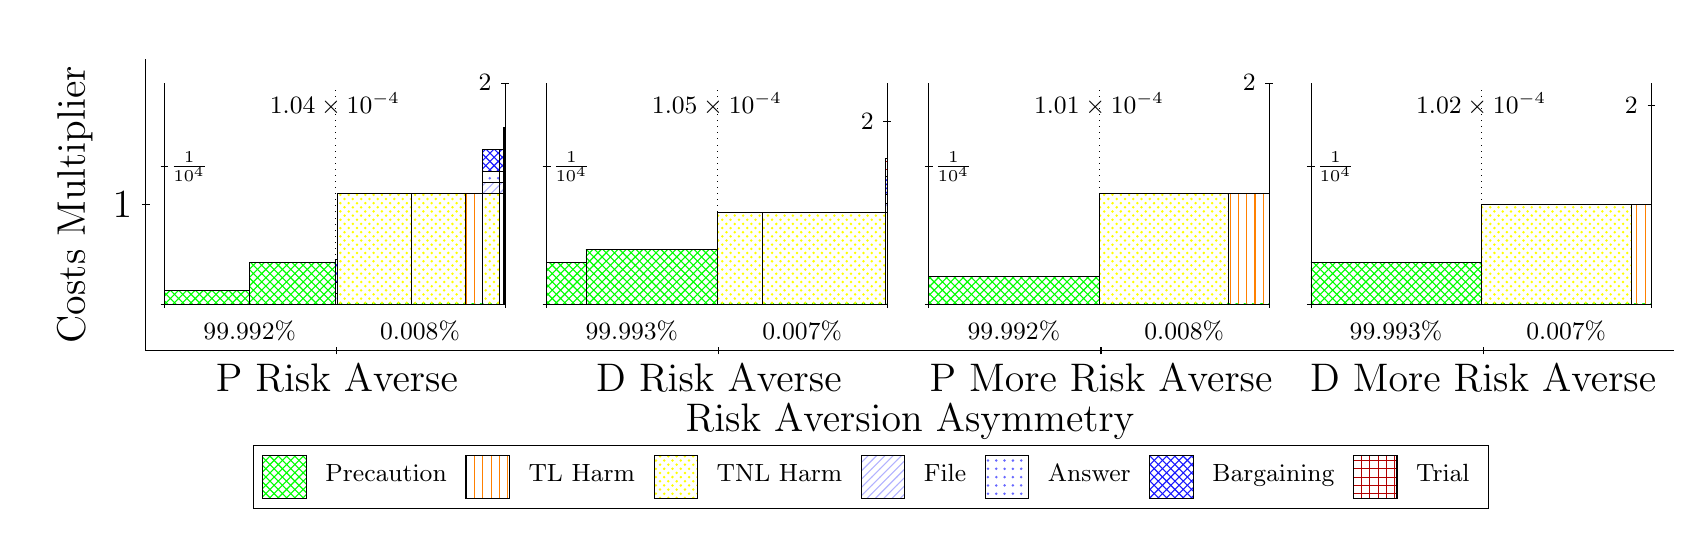
\begin{tikzpicture}
\clip(-0.5,-1.1) rectangle +(20.91,6.2);
\draw[black] (1,1) -- (1,4.7);
\node[rotate=90, fontscale=2, anchor=center] at (0.1, 2.85) {Costs Multiplier};
\draw[black] (0.95,2.85) -- (1.05,2.85);
\node[fontscale=2, anchor=east] at (0.95, 2.85) {1};

\draw[black] (1,1) -- (20.41,1);
\node[fontscale=2, anchor=center] at (10.705, 0.1) {Risk Aversion Asymmetry};
\draw[black] (3.4263,0.95) -- (3.4263,1.05);
\node[fontscale=2, anchor=north] at (3.4263, 0.95) {P Risk Averse};
\draw[black] (8.2788,0.95) -- (8.2788,1.05);
\node[fontscale=2, anchor=north] at (8.2788, 0.95) {D Risk Averse};
\draw[black] (13.131,0.95) -- (13.131,1.05);
\node[fontscale=2, anchor=north] at (13.131, 0.95) {P More Risk Averse};
\draw[black] (17.984,0.95) -- (17.984,1.05);
\node[fontscale=2, anchor=north] at (17.984, 0.95) {D More Risk Averse};


\draw[pattern=crosshatch, pattern color=green,draw=black,very thin] (1.2381,1.592) rectangle (2.3197,1.7662);
\draw[pattern=crosshatch, pattern color=green,draw=black,very thin] (2.3197,1.592) rectangle (3.4013,2.1146);
\draw[pattern=crosshatch, pattern color=green,draw=black,very thin] (3.4013,1.592) rectangle (3.431,1.592);
\draw[pattern=north east lines, pattern color=blue!30,draw=black,very thin] (3.4013,1.592) rectangle (3.431,1.7324);
\draw[pattern=dots,  pattern color=blue!60,draw=black,very thin] (3.4013,1.7324) rectangle (3.431,1.8728);
\draw[pattern=crosshatch,      pattern color=blue!90,draw=black,very thin] (3.4013,1.8728) rectangle (3.431,2.1536);
\draw[pattern=crosshatch, pattern color=green,draw=black,very thin] (3.431,1.592) rectangle (3.4332,1.592);
\draw[pattern=north east lines, pattern color=blue!30,draw=black,very thin] (3.431,1.592) rectangle (3.4332,1.7324);
\draw[pattern=dots,  pattern color=blue!60,draw=black,very thin] (3.431,1.7324) rectangle (3.4332,1.8728);
\draw[pattern=crosshatch,      pattern color=blue!90,draw=black,very thin] (3.431,1.8728) rectangle (3.4332,2.1536);
\draw[pattern=grid,            pattern color=red!70!black,draw=black,very thin] (3.431,2.1536) rectangle (3.4332,2.4344);
\draw[pattern=crosshatch, pattern color=green,draw=black,very thin] (3.4332,1.592) rectangle (4.3686,1.592);
\draw[pattern=crosshatch dots, pattern color=yellow,draw=black,very thin] (3.4332,1.592) rectangle (4.3686,2.996);
\draw[pattern=crosshatch, pattern color=green,draw=black,very thin] (4.3686,1.592) rectangle (4.3762,1.592);
\draw[pattern=vertical lines, pattern color=orange,draw=black,very thin] (4.3686,1.592) rectangle (4.3762,2.996);
\draw[pattern=crosshatch, pattern color=green,draw=black,very thin] (4.3762,1.592) rectangle (5.0554,1.592);
\draw[pattern=crosshatch dots, pattern color=yellow,draw=black,very thin] (4.3762,1.592) rectangle (5.0554,2.996);
\draw[pattern=crosshatch, pattern color=green,draw=black,very thin] (5.0554,1.592) rectangle (5.2782,1.592);
\draw[pattern=vertical lines, pattern color=orange,draw=black,very thin] (5.0554,1.592) rectangle (5.2782,2.996);
\draw[pattern=crosshatch, pattern color=green,draw=black,very thin] (5.2782,1.592) rectangle (5.4887,1.592);
\draw[pattern=crosshatch dots, pattern color=yellow,draw=black,very thin] (5.2782,1.592) rectangle (5.4887,2.996);
\draw[pattern=north east lines, pattern color=blue!30,draw=black,very thin] (5.2782,2.996) rectangle (5.4887,3.1364);
\draw[pattern=dots,  pattern color=blue!60,draw=black,very thin] (5.2782,3.1364) rectangle (5.4887,3.2768);
\draw[pattern=crosshatch,      pattern color=blue!90,draw=black,very thin] (5.2782,3.2768) rectangle (5.4887,3.5576);
\draw[pattern=crosshatch, pattern color=green,draw=black,very thin] (5.4887,1.592) rectangle (5.545,1.592);
\draw[pattern=vertical lines, pattern color=orange,draw=black,very thin] (5.4887,1.592) rectangle (5.545,2.996);
\draw[pattern=north east lines, pattern color=blue!30,draw=black,very thin] (5.4887,2.996) rectangle (5.545,3.1364);
\draw[pattern=dots,  pattern color=blue!60,draw=black,very thin] (5.4887,3.1364) rectangle (5.545,3.2768);
\draw[pattern=crosshatch,      pattern color=blue!90,draw=black,very thin] (5.4887,3.2768) rectangle (5.545,3.5576);
\draw[pattern=crosshatch, pattern color=green,draw=black,very thin] (5.545,1.592) rectangle (5.5515,1.592);
\draw[pattern=crosshatch dots, pattern color=yellow,draw=black,very thin] (5.545,1.592) rectangle (5.5515,2.996);
\draw[pattern=north east lines, pattern color=blue!30,draw=black,very thin] (5.545,2.996) rectangle (5.5515,3.1364);
\draw[pattern=dots,  pattern color=blue!60,draw=black,very thin] (5.545,3.1364) rectangle (5.5515,3.2768);
\draw[pattern=crosshatch,      pattern color=blue!90,draw=black,very thin] (5.545,3.2768) rectangle (5.5515,3.5576);
\draw[pattern=grid,            pattern color=red!70!black,draw=black,very thin] (5.545,3.5576) rectangle (5.5515,3.8384);
\draw[pattern=crosshatch, pattern color=green,draw=black,very thin] (5.5515,1.592) rectangle (5.5644,1.592);
\draw[pattern=vertical lines, pattern color=orange,draw=black,very thin] (5.5515,1.592) rectangle (5.5644,2.996);
\draw[pattern=north east lines, pattern color=blue!30,draw=black,very thin] (5.5515,2.996) rectangle (5.5644,3.1364);
\draw[pattern=dots,  pattern color=blue!60,draw=black,very thin] (5.5515,3.1364) rectangle (5.5644,3.2768);
\draw[pattern=crosshatch,      pattern color=blue!90,draw=black,very thin] (5.5515,3.2768) rectangle (5.5644,3.5576);
\draw[pattern=grid,            pattern color=red!70!black,draw=black,very thin] (5.5515,3.5576) rectangle (5.5644,3.8384);
\node[font=\small,text=black,anchor=north] at (3.4013, 4.4) {$1.04\times 10^{-4}$};
\draw[black,very thin] (1.2381,1.592) -- (1.2381,4.4);
\draw[black,very thin] (1.1881,1.592) -- (1.2881,1.592);
\node[font=\small,text=black, anchor=west] at (1.1881, 1.592) {};
\draw[black,very thin] (1.1881,3.334) -- (1.2881,3.334);
\node[font=\small,text=black, anchor=west] at (1.1881, 3.334) {$\frac{1}{10^{4}}$};

\draw[black,dotted,very thin] (3.4013,1.6762) -- (3.4013,4.3158);
\draw[black,very thin] (5.5644,1.592) -- (5.5644,4.4);
\draw[black,very thin] (5.5144,4.4) -- (5.6144,4.4);
\node[font=\small,text=black, anchor=east] at (5.5144, 4.4) {\contour{white}{2}};

\draw[black,very thin] (1.2381,1.592) -- (5.5644,1.592);
\draw[black,very thin] (1.2381,1.542) -- (1.2381,1.642);
\node[font=\small,text=black, anchor=north] at (1.2381, 1.542) {};
\draw[black,very thin] (5.5644,1.542) -- (5.5644,1.642);
\node[font=\small,text=black, anchor=north] at (5.5644, 1.542) {};

\node[font=\small,text=black,anchor=south] at (2.3197, 0.992) {99.992\%};
\node[font=\small,text=black,anchor=south] at (4.4828, 0.992) {0.008\%};

\draw[pattern=crosshatch, pattern color=green,draw=black,very thin] (6.0906,1.592) rectangle (6.5882,2.1146);
\draw[pattern=crosshatch, pattern color=green,draw=black,very thin] (6.5882,1.592) rectangle (8.2538,2.2888);
\draw[pattern=crosshatch, pattern color=green,draw=black,very thin] (8.2538,1.592) rectangle (8.2547,1.592);
\draw[pattern=north east lines, pattern color=blue!30,draw=black,very thin] (8.2538,1.592) rectangle (8.2547,1.708);
\draw[pattern=dots,  pattern color=blue!60,draw=black,very thin] (8.2538,1.708) rectangle (8.2547,1.8239);
\draw[pattern=crosshatch,      pattern color=blue!90,draw=black,very thin] (8.2538,1.8239) rectangle (8.2547,2.0557);
\draw[pattern=crosshatch, pattern color=green,draw=black,very thin] (8.2547,1.592) rectangle (8.2576,1.592);
\draw[pattern=north east lines, pattern color=blue!30,draw=black,very thin] (8.2547,1.592) rectangle (8.2576,1.708);
\draw[pattern=dots,  pattern color=blue!60,draw=black,very thin] (8.2547,1.708) rectangle (8.2576,1.8239);
\draw[pattern=crosshatch,      pattern color=blue!90,draw=black,very thin] (8.2547,1.8239) rectangle (8.2576,2.0557);
\draw[pattern=grid,            pattern color=red!70!black,draw=black,very thin] (8.2547,2.0557) rectangle (8.2576,2.2876);
\draw[pattern=crosshatch, pattern color=green,draw=black,very thin] (8.2576,1.592) rectangle (8.8286,1.592);
\draw[pattern=crosshatch dots, pattern color=yellow,draw=black,very thin] (8.2576,1.592) rectangle (8.8286,2.7513);
\draw[pattern=crosshatch, pattern color=green,draw=black,very thin] (8.8286,1.592) rectangle (10.389,1.592);
\draw[pattern=crosshatch dots, pattern color=yellow,draw=black,very thin] (8.8286,1.592) rectangle (10.389,2.7513);
\draw[pattern=crosshatch, pattern color=green,draw=black,very thin] (10.389,1.592) rectangle (10.395,1.592);
\draw[pattern=crosshatch dots, pattern color=yellow,draw=black,very thin] (10.389,1.592) rectangle (10.395,2.7513);
\draw[pattern=north east lines, pattern color=blue!30,draw=black,very thin] (10.389,2.7513) rectangle (10.395,2.8672);
\draw[pattern=dots,  pattern color=blue!60,draw=black,very thin] (10.389,2.8672) rectangle (10.395,2.9831);
\draw[pattern=crosshatch,      pattern color=blue!90,draw=black,very thin] (10.389,2.9831) rectangle (10.395,3.215);
\draw[pattern=crosshatch, pattern color=green,draw=black,very thin] (10.395,1.592) rectangle (10.417,1.592);
\draw[pattern=crosshatch dots, pattern color=yellow,draw=black,very thin] (10.395,1.592) rectangle (10.417,2.7513);
\draw[pattern=north east lines, pattern color=blue!30,draw=black,very thin] (10.395,2.7513) rectangle (10.417,2.8672);
\draw[pattern=dots,  pattern color=blue!60,draw=black,very thin] (10.395,2.8672) rectangle (10.417,2.9831);
\draw[pattern=crosshatch,      pattern color=blue!90,draw=black,very thin] (10.395,2.9831) rectangle (10.417,3.215);
\draw[pattern=grid,            pattern color=red!70!black,draw=black,very thin] (10.395,3.215) rectangle (10.417,3.4468);
\node[font=\small,text=black,anchor=north] at (8.2538, 4.4) {$1.05\times 10^{-4}$};
\draw[black,very thin] (6.0906,1.592) -- (6.0906,4.4);
\draw[black,very thin] (6.0406,1.592) -- (6.1406,1.592);
\node[font=\small,text=black, anchor=west] at (6.0406, 1.592) {};
\draw[black,very thin] (6.0406,3.334) -- (6.1406,3.334);
\node[font=\small,text=black, anchor=west] at (6.0406, 3.334) {$\frac{1}{10^{4}}$};

\draw[black,dotted,very thin] (8.2538,1.6762) -- (8.2538,4.3158);
\draw[black,very thin] (10.417,1.592) -- (10.417,4.4);
\draw[black,very thin] (10.367,3.9105) -- (10.467,3.9105);
\node[font=\small,text=black, anchor=east] at (10.367, 3.9105) {\contour{white}{2}};

\draw[black,very thin] (6.0906,1.592) -- (10.417,1.592);
\draw[black,very thin] (6.0906,1.542) -- (6.0906,1.642);
\node[font=\small,text=black, anchor=north] at (6.0906, 1.542) {};
\draw[black,very thin] (10.417,1.542) -- (10.417,1.642);
\node[font=\small,text=black, anchor=north] at (10.417, 1.542) {};

\node[font=\small,text=black,anchor=south] at (7.1722, 0.992) {99.993\%};
\node[font=\small,text=black,anchor=south] at (9.3353, 0.992) {0.007\%};

\draw[pattern=crosshatch, pattern color=green,draw=black,very thin] (10.943,1.592) rectangle (13.106,1.9404);
\draw[pattern=crosshatch, pattern color=green,draw=black,very thin] (13.106,1.592) rectangle (14.743,1.592);
\draw[pattern=crosshatch dots, pattern color=yellow,draw=black,very thin] (13.106,1.592) rectangle (14.743,2.9958);
\draw[pattern=crosshatch, pattern color=green,draw=black,very thin] (14.743,1.592) rectangle (15.269,1.592);
\draw[pattern=vertical lines, pattern color=orange,draw=black,very thin] (14.743,1.592) rectangle (15.269,2.9958);
\node[font=\small,text=black,anchor=north] at (13.106, 4.4) {$1.01\times 10^{-4}$};
\draw[black,very thin] (10.943,1.592) -- (10.943,4.4);
\draw[black,very thin] (10.893,1.592) -- (10.993,1.592);
\node[font=\small,text=black, anchor=west] at (10.893, 1.592) {};
\draw[black,very thin] (10.893,3.334) -- (10.993,3.334);
\node[font=\small,text=black, anchor=west] at (10.893, 3.334) {$\frac{1}{10^{4}}$};

\draw[black,dotted,very thin] (13.106,1.6762) -- (13.106,4.3158);
\draw[black,very thin] (15.269,1.592) -- (15.269,4.4);
\draw[black,very thin] (15.219,4.3996) -- (15.319,4.3996);
\node[font=\small,text=black, anchor=east] at (15.219, 4.3996) {\contour{white}{2}};

\draw[black,very thin] (10.943,1.592) -- (15.269,1.592);
\draw[black,very thin] (10.943,1.542) -- (10.943,1.642);
\node[font=\small,text=black, anchor=north] at (10.943, 1.542) {};
\draw[black,very thin] (15.269,1.542) -- (15.269,1.642);
\node[font=\small,text=black, anchor=north] at (15.269, 1.542) {};

\node[font=\small,text=black,anchor=south] at (12.025, 0.992) {99.992\%};
\node[font=\small,text=black,anchor=south] at (14.188, 0.992) {0.008\%};

\draw[pattern=crosshatch, pattern color=green,draw=black,very thin] (15.796,1.592) rectangle (17.959,2.1146);
\draw[pattern=crosshatch, pattern color=green,draw=black,very thin] (17.959,1.592) rectangle (19.869,1.592);
\draw[pattern=crosshatch dots, pattern color=yellow,draw=black,very thin] (17.959,1.592) rectangle (19.869,2.8534);
\draw[pattern=crosshatch, pattern color=green,draw=black,very thin] (19.869,1.592) rectangle (20.122,1.592);
\draw[pattern=vertical lines, pattern color=orange,draw=black,very thin] (19.869,1.592) rectangle (20.122,2.8534);
\node[font=\small,text=black,anchor=north] at (17.959, 4.4) {$1.02\times 10^{-4}$};
\draw[black,very thin] (15.796,1.592) -- (15.796,4.4);
\draw[black,very thin] (15.746,1.592) -- (15.846,1.592);
\node[font=\small,text=black, anchor=west] at (15.746, 1.592) {};
\draw[black,very thin] (15.746,3.334) -- (15.846,3.334);
\node[font=\small,text=black, anchor=west] at (15.746, 3.334) {$\frac{1}{10^{4}}$};

\draw[black,dotted,very thin] (17.959,1.6762) -- (17.959,4.3158);
\draw[black,very thin] (20.122,1.592) -- (20.122,4.4);
\draw[black,very thin] (20.072,4.1148) -- (20.172,4.1148);
\node[font=\small,text=black, anchor=east] at (20.072, 4.1148) {\contour{white}{2}};

\draw[black,very thin] (15.796,1.592) -- (20.122,1.592);
\draw[black,very thin] (15.796,1.542) -- (15.796,1.642);
\node[font=\small,text=black, anchor=north] at (15.796, 1.542) {};
\draw[black,very thin] (20.122,1.542) -- (20.122,1.642);
\node[font=\small,text=black, anchor=north] at (20.122, 1.542) {};

\node[font=\small,text=black,anchor=south] at (16.877, 0.992) {99.993\%};
\node[font=\small,text=black,anchor=south] at (19.04, 0.992) {0.007\%};

\coordinate (LegendAnchor) at (10.205000000000002,0);
\begin{scope}[align=center]
\matrix[scale=0.6,draw=black,below=0.2cm of LegendAnchor,nodes={draw},column sep=0.12cm]{
\node[rectangle,draw,minimum width=0.55cm,minimum height=0.55cm,pattern=crosshatch, pattern color=green]{}; &
        \node[draw=none,font=\small]{Precaution}; &
\node[rectangle,draw,minimum width=0.55cm,minimum height=0.55cm,pattern=vertical lines, pattern color=orange]{}; &
        \node[draw=none,font=\small]{TL Harm}; &
\node[rectangle,draw,minimum width=0.55cm,minimum height=0.55cm,pattern=crosshatch dots, pattern color=yellow]{}; &
        \node[draw=none,font=\small]{TNL Harm}; &
\node[rectangle,draw,minimum width=0.55cm,minimum height=0.55cm,pattern=north east lines, pattern color=blue!30]{}; &
        \node[draw=none,font=\small]{File}; &
\node[rectangle,draw,minimum width=0.55cm,minimum height=0.55cm,pattern=dots, pattern color=blue!60]{}; &
        \node[draw=none,font=\small]{Answer}; &
\node[rectangle,draw,minimum width=0.55cm,minimum height=0.55cm,pattern=crosshatch, pattern color=blue!90]{}; &
        \node[draw=none,font=\small]{Bargaining}; &
\node[rectangle,draw,minimum width=0.55cm,minimum height=0.55cm,pattern=grid, pattern color=red!70!black]{}; &
        \node[draw=none,font=\small]{Trial}; \\
};\end{scope}

\end{tikzpicture}
\end{document}